\documentclass[../main.tex]{subfiles}
\begin{document}
	\chapter{Espaços Vetoriais}
	\begin{description}
		\item[Videoaula 12 - Espaços Vetoriais] \hfill \\
		\url{https://www.youtube.com/watch?v=UkKQEYRdiks}
		
		\item[Videoaula 18 - Espaços Vetoriais Abstratos] \hfill \\
		\url{https://www.youtube.com/watch?v=dkaUQG1Ic3A}
		
		\item[Videoaula 13 - Subespaços Vetoriais] \hfill \\
		\url{https://www.youtube.com/watch?v=4D-q8OIXa94}
		
		\item[Videoaula 16 - Base e Dimensão] \hfill \\
		\url{https://www.youtube.com/watch?v=wSXwQ3gM7Eo}
		
		\item[Videoaula 17 - Coordenadas] \hfill \\
		\url{https://www.youtube.com/watch?v=GPnZsHawg6A}
		
		\item[Videoaula 20 - Ortogonalidade] \hfill \\ \url{https://www.youtube.com/watch?v=QxsxaQrCHww}
		
		\item[Videoaula 21 - Processo de Ortogonalização de Gram-Schmidt ] \hfill \\
		\url{https://www.youtube.com/watch?v=GbQ-pjpsY9Q}
		
		
	\end{description}
	
	\newpage
	
	\section{Espaços Vetoriais}
	Espaços vetoriais são, basicamente, a nossa bancada de trabalho, e os vetores, as ferramentas com as quais construímos muitas funcionalidades. Exemplos disso são as LLMs (ChatGPT, Gemini, DeepSeek) e os sites de busca (Google, DuckDuckGo). Eles utilizam vetores para executar suas tarefas: todas as entradas são convertidas para dentro de um espaço vetorial e, de acordo com a posição do seu vetor, o sistema aproxima os resultados mais relevantes para você.
	
	Além das aplicações na vida real, também temos na matemática pura, espaços vetoriais são muito necessário em cálculo de múltiplas variáveis e uma das bases de análise funcional.
	
	\begin{definicao}
		\azul{Espaços vetorial} é um conjunto $V$ não vazio no qual existe as operações de adição (entre vetores) e multiplicação por um número real (escalar), respeitando as seguintes propriedades com as operações citadas, sendo $u$, $v$ e $w$ vetores e $\alpha$ e $\beta$ escalares:
		
			\begin{description}
				% O \item[] cria o título da categoria
				\item[Adição:] \hfill 
				\begin{enumerate}
					\item[(A1)] $u + v = v + u$ (Comutatividade);
					\item[(A2)] $(u + v) + w = u + (v + w)$ (Associatividade);
					\item[(A3)] $ \exists v : v + u = u + v = u $ denotamos $v$ por $\vec{0}$ (Vetor nulo);
					\item[(A4)] $\forall u \, \, \exists v : u + v = v + u = \vec{0}$ denotamos $v$ por $-u$ (Inverso aditivo).
				\end{enumerate}
				
				\item[Multiplicação por Escalar:] \hfill 
				\begin{enumerate}
					\item[(M1)] $\alpha(u + v) = \alpha u + \alpha v$ (Distributividade de um escalar);
					\item[(M2)] $(\alpha + \beta)v = \alpha v + \beta v$ (Distributividade de um vetor);
					\item[(M3)] $v \cdot 1 = v$ (Multiplicação por 1);
					\item[(M4)] $\alpha (\beta \cdot v) = (\alpha \cdot \beta)v$ (Associatividade).
				\end{enumerate}
			\end{description}
	\end{definicao}
	\begin{definicao}
		Elementos de um espaço vetorial $V$ são denominados \azul{vetores}.
	\end{definicao}
	\begin{exemplo}[Espaço real - $\mathbb{R}^n$] O plano euclidiano de dimensão n ($\mathbb{R}^n$) é um dos exemplos mais clássicos de espaço vetorial, seja dois vetores $u=(\eta_1,...,\eta_n)$ e $v=(\delta_1,...,\delta_n)$ e também $\alpha$ sendo escalar, com sua soma e multiplicação definido por:
	\begin{align*}
		u + v &= (\eta_1 + \delta_1, \dots , \eta_n + \delta_n) \\
		\alpha \cdot u &= (\alpha \eta_1, \dots, \alpha \eta_n)
	\end{align*}
	\begin{center}
		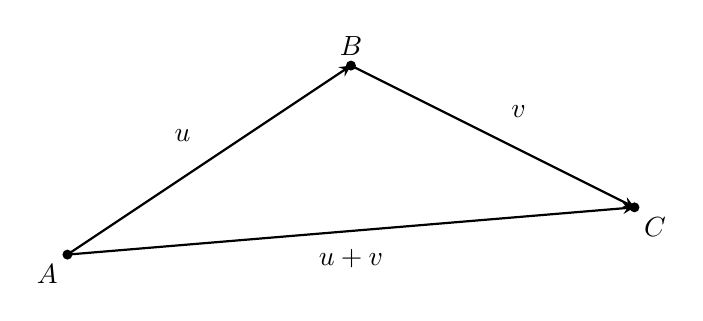
\begin{tikzpicture}[scale=1.2, >=stealth]
			% Pontos
			\coordinate (A) at (0,0);
			\coordinate (B) at (3,2);
			\coordinate (C) at (6,0.5);
			
			% Lados com setas
			\draw[thick, ->] (A) -- (B) node[midway, above left=3pt] {$u$};
			\draw[thick, ->] (B) -- (C) node[midway, above right=3pt] {$v$};
			\draw[thick, ->] (A) -- (C) node[midway, below=3pt] {$u+v$};
			
			% Pontos marcados
			\fill (A) circle (1.5pt) node[below left] {$A$};
			\fill (B) circle (1.5pt) node[above] {$B$};
			\fill (C) circle (1.5pt) node[below right] {$C$};
		\end{tikzpicture}\\
		(Exemplo no $\mathbb{R}^2$)
		\end{center}
		\end{exemplo}
		\begin{exemplo}[Espaço de matrizes $n \times m$]
			O conjunto das matrizes $n\times m$ com soma entre vetores e multiplicação por escalar definido da seguinte forma:
			\begin{description}
					\item \[
					\begin{bmatrix}
						a_{11} & a_{12} & ... & a_{1m}  \\
						a_{21} & a_{22} & ... & a_{2m} \\
						... & ... & ... & ... \\
						a_{n1} & a_{n2} & ... & a_{nm}
					\end{bmatrix} + \begin{bmatrix}
					b_{11} & b_{12} & ... & b_{1m}  \\
					b_{21} & b_{22} & ... & b_{2m} \\
					... & ... & ... & ... \\
					b_{n1} & b_{n2} & ... & b_{nm}
					\end{bmatrix} = \begin{bmatrix}
					(a+b)_{11} & (a+b)_{12} & ... & (a+b)_{1m}  \\
					(a+b)_{21} & (a+b)_{22} & ... & (a+b)_{2m} \\
					... & ... & ... & ... \\
					(a+b)_{n1} & (a+b)_{n2} & ... & (a+b)_{nm}
					\end{bmatrix}
					\]
					\item \[\alpha \begin{bmatrix}
						a_{11} & a_{12} & ... & a_{1m}  \\
						a_{21} & a_{22} & ... & a_{2m} \\
						... & ... & ... & ... \\
						a_{n1} & a_{n2} & ... & a_{nm}
					\end{bmatrix} = \begin{bmatrix}
					(\alpha a)_{11} & (\alpha a)_{12} & ... & (\alpha a)_{1m}  \\
					(\alpha a)_{21} & (\alpha a)_{22} & ... & (\alpha a)_{2m} \\
					... & ... & ... & ... \\
					(\alpha a)_{n1} & (\alpha a)_{n2} & ... & (\alpha a)_{nm}
					\end{bmatrix}
					\]
			\end{description}
			é um espaço vetorial, chamado de espaço vetorial da matrizes $n\times m$.
		\end{exemplo} \bigskip
		{\Large\textbf{Exercícios}}
		\begin{enumerate}
			\item Descreva o vetor nulo dos seguintes espaços vetoriais, considerando as operações usuais: \hfill 
			\begin{center}
				a)$\mathbb{R}^5$ \hspace{4cm} b)$\mathbb{M}_{3\times 2}$ \hspace{4cm}
			\end{center}
			\item Mostre que o espaço $\mathbb{P}_n = p(x) = a_0 + a_1 x + a_2 x^2 + ... + a_n x^n : a_0, a_1, a_2, a_3, ..., a_n \in \mathbb{R}$ dos
			polinômios reais de grau menor ou igual a $n$ é um espaço vetorial real, com as operações usuais de soma e multiplicação por escalar.
			\item Verifique se $V = {x \in \mathbb{R}: x > 0}$ é um espaço vetorial com as operações de adição ($\oplus$) e a multiplicação por escalar ($\odot$) dadas abaixo. Em caso positivo, prove e indique o vetor nulo (neutro aditivo) e o inverso aditivo.
			\begin{center}
				$x \oplus y = xy$ \hspace{1cm} e \hspace{1cm} $\alpha \cdot x = x^\alpha$
			\end{center}
		\end{enumerate} 
		\newpage
	\section{Subespaços Vetoriais}
		Subespaços vetoriais são subconjuntos de um espaço vetorial maior que ainda utilizam das mesmas operações e são ''independentes'' do espaço vetorial original, sendo mais exato:
		\begin{definicao}
			Seja $E$ um espaço vetorial. Um \azul{subespaço vetorial} (ou simplesmente \azul{subespaço}) de $E$ é um subconjunto $F \subset E$ com as seguintes propriedades:
				\begin{enumerate}
				\item[(P1)] $\vec{0} \in F$;
				\item[(P2)] Se $u, v \in F$ então $u+v \in F$;
				\item[(P3)] Se $v \in F$ então, para todo $\alpha \in \mathbb{R}$, $\alpha v \in F$.
			\end{enumerate}
		\end{definicao}
		Decorrendo da definição, percebemos que todo subespaço é um espaço vetorial em si mesmo, também percebemos que em todo espaço vetorial existe o \azul{subespaço trivial}, composto somente pelo vetor nulo.\\ \bigskip
		
		{\Large\textbf{Exercícios}}
		\begin{enumerate}
				\item Prove que um plano é um subespaço vetorial de $\mathbb{R}^3$ se, e somente se, o plano passa pela origem.
				\item Sejam $A_{m\times n}$ e $B_{n \times 1}$ matrizes. Prove que o conjunto solução de $AX = B$ é subespaço vetorial de $M_{n\times 1}$ se, e somente se, $B = 0$.
		\end{enumerate}
	
	\section{Base, Dimensão e Coordenadas}
	
	
	Os espaços vetoriais de dimensão finita (finitas coordenadas) são composto por uma estrutura algébrica simples, sendo principalmente evidenciados pelo conceito de base. Pense como a base sendo um gerador de espaços vetoriais, assim como um vetor (ou dois vetores) no $\mathbb{R}^n$ geram uma reta (ou um plano) é possível expandir isso para dimensões maiores ou outros conceitos utilizando de bases.
	
	Recapitulando os conceitos da seção 2.3, mas agora com uma noção vetorial ao invés de matricial, temos que:
	\begin{definicao}
		Seja $E$ um espaço vetorial. Dizemos que $X \subset E$ é \azul{linearmente independente} quando nenhum vetor $v \in X$ é combinação linear de outros elementos de $X$. 
	\end{definicao}
	
	\textbf{Observação.} Perceba que dessa definição temos que caso $\vec{0}$ esteja no subconjunto $X$ teremos consequentemente que $X$ é L.D., pois $\vec{0}$ pode ser gerado por quaisquer combinação linear que seus coeficientes sejam todos nulos.
	
	$$\vec{0}=0\cdot v_1 + ... + 0\cdot v_m $$
	
	\begin{definicao}
		Dizemos que $X$ é \azul{linearmente dependente} quando \textbf{não é linearmente independente}.
	\end{definicao}
	
	Fazendo ainda conexão com a seção 2.3, temos o seguinte teorema que faz a ligação com matrizes:
	
	\begin{teorema}
		Seja $X$ um subconjunto no espaço vetorial $E$. Se a única combinação linear de $X$ que gera o vetor nulo é aquela cujos coeficientes são todos iguais a zero, então $X$ é L.I.
	\end{teorema}
	
	\textbf{Prova.} Suponha por absurdo que se tenha coeficientes nem todos nulos que podemos ter $\alpha_1 v_1 + ... + \alpha_m v_m = 0$ com $v_1, ..., v_m \in X$. Vamos supor que $\alpha_1 \neq 0$ por via de simplicidade. Então temos que $v_1 = -(\frac{\alpha_2}{\alpha_1})v_2 - ... -(\frac{\alpha_m}{\alpha_1})v_m = 0$, o que deixa $v_1$ como combinação linear de outros elementos de $X$. \qed
	\smallskip
	\begin{exemplo}[Vetores canônicos]Os vetores canônicos no $\mathbb{R}^n$ são L.I., basta observar que cada vetor difere um do outro em duas coordenadas, pegue $e_1 = (1,0,0)$, $e_2 = (0,1,0)$ e $e_3 = (0,0,1)$ no $\mathbb{R}^3$ por exemplo, teremos que é impossível formar uma combinação linear de um a partir do outro.
	\end{exemplo}
	
	\begin{definicao}
		Dizemos que o conjunto $\mathcal{B}$ é uma \azul{base} do espaço vetorial $E$ se:
		\begin{enumerate}[itemsep=0pt]
			\item $\mathcal{B} \subset E$;
			\item $\mathcal{B}$ é L.I;
			\item $\mathcal{B}$ gera o espaço vetorial $E$.
		\end{enumerate}
	\end{definicao}
	
	\textbf{Observação.} Isto significa que todos os vetores de $E$ podem ser reescritos como combinação linear dos vetores da base $\mathcal{B}$ de $E$. Volto a trazer o que foi falado antes da reta e do plano, podemos representar todos os vetores de um plano como combinação linear de dois vetores não paralelos desse mesmo plano, o mesmo ocorre com o $\mathbb{R}^3$, mas com 3 vetores não coplanares.
	\smallskip
		
	\begin{definicao}
		Se $\mathcal{B}$ é uma base de $E$ e $w$ é um vetor formado pela combinação linear $\alpha_1 v_1 + ... + \alpha_m v_m$ com $v_1, ..., v_m \in \mathcal{B}$ então dizemos que $\alpha_1, ..., \alpha_m$ são as \azul{coordenadas} de $w$.
	\end{definicao}
	
	\textbf{Observação.} Também pode ser reinterpretado como os coeficientes dados aos vetores da base para se obter o vetor $w$.
	\smallskip
	
	\begin{definicao}
		A \azul{dimensão} de um espaço vetorial é a cardinalidade de alguma base desse mesmo espaço, ou seja, a quantidade de elementos que uma base desse espaço tem.
	\end{definicao}
	
	Com o teorema 1.3.8. veremos que podemos sim escolher qualquer base para obtermos a dimensão de um espaço vetorial, por conta que todas as bases de um mesmo espaço vetorial obtém de uma mesma quantidade de elementos. Também sendo um dos teoremas mais importante no conteúdo de bases, com ele decorre 3 corolários importantíssimos.
	
	\smallskip
	
	\textbf{Lema.} Todo sistema linear homogêneo que o número de incógnitas é maior do que o número de equações admite uma solução não trivial.
	\\ \smallskip
	\textbf{Prova:} Use o teorema 2.2.18. \qed
	\smallskip
	
	\begin{teorema}
		Se os vetores $v_1, ..., v_m$ geram o espaço vetorial $E$ então qualquer conjunto com mais de $m$ vetores em $E$ é L.D.
	\end{teorema}
	\textbf{Prova:} Dados os vetores $w_1, ..., w_n$ em $E$, com $n > m$, para cada $j = 1, ..., n$ temos $w_j = \alpha_{1j}v_1 + ... + \alpha_{mj}v_m$ pois os vetores $v_1,...,v_m$ geram $E$. Para mostrar que os vetores $w_j$ são L.D., devemos achar coeficientes $x_1, ..., x_n$, não todos iguais a zero, tais que $x_1w_1+...+x_nw_n=0$. Substituindo os $w_j$ por suas expressões em termos dos $v_i$, esta igualdade significa que
	$$\left(\sum_{j=1}^{n}x_j\alpha_{1j}\right)v_1+...+\left(\sum_{j=1}^{n}x_j\alpha_{mj}\right)v_m = 0$$
	Certamente esta última condição será satisfeita desde que todos os somatórios dentro dos parênteses sejam nulos, ou seja, que $(x_1, ..., x_n)$ seja uma solução não trivial do sistema homogêneo 
	$$\alpha_{11}x_1+...+\alpha_{1n}x_n = 0$$
	$$\alpha_{21}x_1+...+\alpha_{2n}x_n = 0$$
	$$\vdots$$
	$$\alpha_{m1}x_1+...+\alpha_{mn}x_n = 0$$
	Uma tal solução existe pelo lema anterior a esse teorema, pois $n>m$. Logo $w_1, ..., w_n$ são L.D. \qed
	
	Os próximos três corolários decorrem do teorema anterior:
	
	\textbf{Corolário 1.} Se os vetores $v_1, ..., v_m$ geram o espaço vetorial $E$ e os vetores $u_1,...,u_n \in E$ são L.I., então $n\leqslant m$
	\\
	\textbf{Corolário 2.} Se o espaço vetorial $E$ admite uma base $\mathcal{B}={u_1,...,u_n}$ com $n$ elementos, qualquer outra base de $E$ terá também n elementos.
	\\
	\textbf{Corolário 3.} Se a dimensão de $E$ é $n$, um conjunto com $n$ vetores gera $E$ se, e somente se, é L.I. 
	
	
	
	\section{Produto Interno}
	
	\section{Ortogonalidade}
		\subsection{Processo de Ortogonalização de Gram-Schmidt}
	
\end{document}
